\documentclass[sigconf, review=false, anonymous=false]{acmart}

%\documentclass[letterpaper,times,10pt]{article}
%\documentclass[letterpaper,times,10pt,twocolumn]{article}
%\documentclass[conference,letterpaper,10pt,times]{IEEEtran}
%\usepackage[top=.9in,left=1in,right=.9in,bottom=1in]{geometry}
%\usepackage{latex8}
%\usepackage{fullpage}
%\usepackage{cite}
%\usepackage{textcomp}
%\usepackage{mathcomp}
%\usepackage{listings}
%\usepackage{latexsym}
%\usepackage[plain]{algorithm}
%\usepackage{epsfig}
%\usepackage{setspace}
%\usepackage{subfig}
%\usepackage{wrapfig}

\usepackage{times}
\usepackage{amssymb}
\usepackage{amsmath}
%\usepackage[pdftex]{graphicx}
\usepackage{subcaption}
\usepackage{url}
\usepackage{color}
\usepackage{listings}
\usepackage{fancyhdr}
\usepackage{flushend}
\usepackage{xspace}

% Enabling these settings may help prevent bib entries from being split across
% pages and causing LaTeX to keel over
%\clubpenalty=10000
%\widowpenalty=10000

%\lstloadlanguages{C}
%\pagestyle{empty}

%\title{Efficient Runtime Support for a Partitioned Global Logical Address Space}

% \author{
% %\begin{normalsize}
% \begin{tabular}{cc}
% D. Brian Larkins         & James Dinan\\
% Rhodes College          & Intel Corporation\\
% Memphis, TN  38112  & Boston, MA 01234\\
% larkinsb@rhodes.edu  & james.dinan@intel.com\\
% \end{tabular}
% %\end{normalsize}
% }

%\usepackage[
%  pdfborder={0 0 0},
%  colorlinks=false,
%  pdfpagelabels=false,
%  pdftitle={Efficient Runtime Support for a Partitioned Global Logical Address Space},
%  pdfauthor={D. Brian Larkins, John Snyder, and James Dinan},
%  pdfsubject={},
%  pdfkeywords={},
%  bookmarks=false,
%]{hyperref}

\newcommand{\pdht}{{PDHT}\xspace}

%\newcommand{\comment}[1]{}
\newcommand{\code}[1]{{\small\sf #1}}
\newcommand{\note}[2]{\textcolor{red}{\textbf{#1}: #2}}
\newcommand{\othertm}{\textsuperscript{$\star$}\xspace}
\newcommand{\regtm}{\textsuperscript{\textregistered{}}\xspace}
\newcommand{\tm}{{\scriptsize\texttrademark{}}\xspace}


% Document starts
\begin{document}
%\IEEEoverridecommandlockouts

% Title portion
\title{Efficient Runtime Support for a \\Partitioned Global Logical Address Space}

\author{D. Brian Larkins}
\affiliation{
    \institution{Rhodes College}
    \city{Memphis}
    \state{TN}
}
\email{larkinsb@rhodes.edu}

\author{John Snyder}
\affiliation{
    \institution{Rhodes College}
    \city{Memphis}
    \state{TN}
}
\email{snyjm-18@rhodes.edu}

\author{James Dinan}
\affiliation{
    \institution{Intel Corporation}
    \city{Hudson}
    \state{MA}
}
\email{james.dinan@intel.com}


%\author{\IEEEauthorblockN{D. Brian Larkins\IEEEauthorrefmark{1}, John Snyder\IEEEauthorrefmark{2}}
%\IEEEauthorblockA
%\IEEEauthorblockA{Memphis, TN}
%\IEEEauthorblockA{Email: \IEEEauthorrefmark{1}larkinsb@rhodes.edu, \IEEEauthorrefmark{2}snyjm-18@rhodes.edu}
%\and
%\IEEEauthorblockN{James Dinan\IEEEauthorrefmark{3}}
%\IEEEauthorblockA{Intel Corporation}
%\IEEEauthorblockA{Hudson, MA}
%\IEEEauthorblockA{Email: james.dinan@intel.com}
%\thanks{\hspace{-1em}CC/Grid; Washington, D.C.; May 2018\newline
%   5/18/\$31.00 \copyright 2018 IEEE}
%   %978-1-5090-3829-9/16/\$31.00 \copyright 2016 IEEE}
%}


%\lstset{language=C,basicstyle={\tt \scriptsize},framexbottommargin=3pt,emph={gt_group_t,gt_tree_t,gt_visitor_t,gt_node_t,gt_nodeptr_t,gt_visit_node_t,size_t},emphstyle=\bf,framexrightmargin=-5ex,framextopmargin=1.5ex}

\acmConference[ICPP'18]{International Conference on Parallel Processing}{August 2018}{Eugene, OR USA}
\begin{abstract}
This is an abstract abstract.
\end{abstract}


\maketitle

%\doublespacing


\thispagestyle{empty}

\section{Introduction}

Partitioned Global Address Space (PGAS) parallel programming models, such as
OpenSHMEM~\cite{openshmem-1.3}, Unified Parallel C~\cite{upc-13-spec}, Fortran
2008 Coarrays~\cite{reid:08,fortran-2008}, and the MPI Remote Memory Access
(RMA) interface MPI~\cite{mpi-forum:15}, have become popular as a means for
supporting distributed, shared global data.  In particular, PGAS models have
been shown to be especially effective when used to store dense arrays and
several models have been designed to support this type of
data~\cite{ga,kamil:14,ddi,niu:16}.

While PGAS models are commonly used with regularly structured data, they have
had limited success with irregular and sparse data.  Such data structures are
accessed indirectly and an additional indexing operation is needed to resolve
the location of a data element.  Indexing structures grow proportional to the
data size; thus, for the large data volumes that necessitate a PGAS solution, these
structures must also be distributed.  As a result, resolving the index of a data item
within the global address space is not possible using only local information.

Remote direct memory access (RDMA) read, write, and atomic update operations
are commonly supported by the high-speed fabrics used to construct HPC systems
and these operations are used to accelerate remote access operations performed
by PGAS models.  RDMA operations map well to remote array access operations,
since the locations to be accessed can be determined at the initiator of the
operation.  However, the indirect addressing required to remotely access sparse or
irregularly structured data presents challenges to existing RDMA interfaces
and can result in significant overheads.

% many applications that use sparse data structures are naturally expressed
% using logical addresses, such as a coordinate/level system in a spatial
% decompositon tree, etc.

% matching an irregular data structure's logical addressing scheme to a 
% traditional PGAS model can be challenging. 

% drawbacks/challenges with true PGAS models
%    - LA -> PA not feasible (i.e. grandchild of a tree node)
%    - indirections 
%       - (multiple fetches)
%       - directory structures
%    - adds latency for each access
%    - data layout may change over time
%    - caching is no silver bullet

% drawbacks with MPI / message passing approaches
%    - tags can be used to associate "logically addressed" locations
%    - MPI does not provide a fetch/get mechanism to communicate 
%      a tagged location

% this work describes an efficient implementation of a PGLAS system 
% that is built on networking mechanisms designed to support MPI
% communications

% our approach is based on some insights
%   - low-level networking systems provide direct support for
%     logical address systems 
%   - using lower-level systems reduce communication overhead
%   - applications can refer to globally shared data objects
%     using an addressing scheme that corresponds to the problem
%     at hand


% in particular, our work takes advantage of the Portals 4 network
% programming interface. Portals works great for a number of
% HPC communication middleware MPI and PGAS-based systems such as
% OpenMPI and UPC
%
% it's also great that Portals is designed to play nice with
% hardware offload systems

% in this paper we describe the implementation of a system that
% realizes a PGLAS with a PDHT and is implemented using the 
% Portals networking interface
% we make the following contributions:
%  - MPI matching interfaces can be used to implement a PGLAS
%  - PGLAS support can be easily run on hardware offload systems
%    that also support optimized MPI matching operations
%  - relying on the network layer to map matching criteria
%    to phys addr reduces the likelihood for collisions vs
%    a conventional hash table structure


The Portals 4.1 network programming interface~\cite{portals4} provides a
well-known interconnect programming model that is designed to permit efficient
hardware offload of communication processing. For example, the Bull\othertm{}
BXI\othertm{} interconnect~\cite{bxi} provides a hardware accelerated
implementation of the Portals 4.1 interface and the Cray\othertm{}
Seastar\othertm{} interconnect~\cite{brightwell:micro:06} provided a hardware
accelerated implementation of the Portals 3.0 interface.  Parallel programs
written using programming models that are built on the Portals interface will
be able to take advantage of network offload hardware.  The problem, of course,
is to map application-level data and task abstractions onto programming
constructs that are aligned with the communication operations supported by
low-level communications systems. 

Portals is designed as a low-level abstraction layer for the network interface
hardware. The Portals structures and communication operations operations are
meant to support the efficient implementation of high-performance programming
interfaces and runtime systems that provide either message-passing semantics
(such as MPI), or one-sided, partitioned global address (PGAS) support. For
message-passing systems, Portals provides a {\em matching interface} that
allows communication middleware to robustly support a two-sided (matched sends
and receives) communication model. Alternatively, Portals also provides a {\em
non-matching interface} that sheds much of the complexity in matching messages
for efficient handling of one-sided communication operations found in PGAS
systems and languages.

Rather than considering the matching and non-matching interfaces as
the basis for higher-level communication systems, we have developed a
system that provides a distributed key/value storage that use Portals
primitives in a novel manner, leading towards a hardware accelerated
hash table system providing a PGLAS programming model. In this paper, we describe the implementation of a
parallel distributed hash table (PDHT) that is implemented directly
using the Portals programming interface. This work is based on the
following insights: (1) implementing data structures using Portals
leads to an opportunity to leverage efficient, hardware accelerated
implementations of Portals and (2) that operations on a hash-table
can be readily mapped to operations within
Portals that would be difficult to express exclusively within an
MPI-like system or a PGAS system.

This work makes the following contributions: We identify the
logically-addressed PGLAS paradigm as a novel extension to existing PGAS
programming concepts, which improves support for sparse and loosely structured
data.  We demonstrate the utility of this model through two representative
scientific applications, MADNESS and Meraculous, from the computational
chemistry and genomics domains, respectively.  We describe a new PGLAS model,
PDHT, a one-sided distributed hash table that is implemented using a novel
application of Portals matching interface operations. Lastly, we provide an
experimental validation, indicating that this approach can yield significant
performance improvements for these classes of applications.

% high performance interconnect hardware
%  - provides hardware optimized for use cases
%  - matching - > MPI
%  - one-sided PGAS

% insights

% contributions

%%% Local Variables:
%%% mode: latex
%%% TeX-master: "paper"
%%% End:

\section{Background}

In this work, we explore efficient runtime support for partitioned, global
logical address spaces (PGLAS).  We define the PGLAS data model to be similar
to PGAS data models, which have been in use for over two decades, with the
distinction that data elements are logically addressed using an
application-meaningful {\em key}.  Each key is mapped to a partition of the
global address space and an application can query locality information for a
given key or iterate over local keys, e.g., to support owner-computes models of
work distribution.  In contrast, PGAS models traditionally use a direct
addressing model, such as a remote address (OpenSHMEM and UPC), an offset into
a remote buffer (MPI), or an index into a regular array (Fortran Coarrays).
While there are differences in memory addressing and layout, PGLAS utilizes the
same one-sided, asynchronous data access model as existing PGAS approaches and
data in global space is accessed using one-sided get (read), put
(write), and atomic access functions.  Thus, PGLAS is a member of the broader
family of distributed key/value stores where data organization and access are
similar to PGAS models.

Most PGAS models require global knowledge of data layout in order to
communicate efficiently.  For example, in the OpenSHMEM model, the layout of
the globally accessible space must be identical at all processes.  As a result,
management of globally accessible memory must be performed collectively.  In
contrast, PGLAS introduces a layer of indirection that translates logical
addresses to direct addresses.  The introduction of this layer
has the potential to relax the strong memory management semantics required by
most PGAS models, enabling more dynamic usage models.  In particular, PGLAS can
support dynamic insertions and removals of key/value pairs in the global
address space.

Efficient and scalable support for translation of keys to memory locations is a
performance-critical, new requirement imposed by PGLAS.  Traditional one-sided
communication operations can satisfy the one-sided and asynchronous
requirements of key translation.  However, multiple operations are required to
query a remote translation structure, leading to high overheads~\cite{namashivayam:15}.  We observe
that the user-supplied tag used by MPI runtimes to match an incoming message
(i.e., put) with a posted receive operation supports a key/value-like remote
write model.  When MPI message processing is performed directly by the NIC,
this model can be seen to support key/value-style put operations.  However,
there are several key differences between MPI messaging and PGLAS
communication.  First, MPI requires message ordering, whereas PGLAS utilizes
the PGAS unordered-by-default communication model.  Further, when an MPI
runtime receives a message for which there is no matching entry, the message is
treated as unexpected and will be accepted once a matching receive operation is
posted.  In contrast, PGLAS models reject remote accesses to nonexistent keys.
Finally, a posted receive operation is consumed by an incoming message, whereas
a PGLAS model maintains the key/value association until the entry is freed.

% motivation
\subsection{Hash Tables}

Hash tables are one of the most widely used data
structures in sequential programs. Data is stored by mapping a key to
a value. Values may be retrieved in a random access manner by
providing the key to get or put operations on the hash table.
%
% serial vs. parallel approaches
Hash tables can be implemented with a myriad of different techniques,
but are traditionally implemented sequentially as an array of pointers
to objects. Parallel implementations typically distribute table data
across nodes, requiring that the hash table stores the entire object
and not simply a reference.
%
In this work, we explore the implementation of a parallel, distributed hash
table as a first implementation of the PGLAS data model.

% sparsity
\subsection{Sparsity}
Of interest to the HPC community, we see parallel hash tables as a
means for dealing with sparsity. Many common HPC applications rely on
sparse data structures, which causes numerous problems in the hunt for
high performance. Matrix and tensor representations often must contend
with sparse data, resulting in specialized formats such compressed
sparse row (CSR) and variants. Other problems, such as N-body
simulation, grid and mesh solvers, are naturally expressed using
spatial decomposition trees such as quadtrees and octrees. 

In these cases, there is a natural mapping between an index or
coordinate system and the corresponding data. A global distributed
hash table could replace a complicated and difficult to parallelize
sparse data structures given the right application.

\subsection{Related Work}

The idea of logically addressing data across memories in a distributed system
has been explored in a number of other models.  Distributed, shared key/value
stores are an intrinsic part of the Piccolo programming model~\cite{power:10}.
The Linda programming model~\cite{ahuja:86} is build around tuple spaces, which
allow data to be inserted, read, and removed from global memory and data items
are identified through a user-supplied tuple.  Such models are of renewed
interest in the context of resilience~\cite{wilke:14}.  Distributed object
models, such as Orca~\cite{bal:92}, reference shared data through graphs rather
than direct pointers.  In the Open Community Runtime (OCR)~\cite{OCR}, data
blocks (DBs) are identified by a globally unique ID, which is assigned by the
OCR runtime system and used to portably reference a DB.  Finally, migratable
object models, such as Charm++~\cite{kale:93}, support a variety of methods for
representing and querying object collections.

Hash tables are also commonly used to store sparse or loosely structured data
and they have been studied in the context of MPI and popular PGAS
models~\cite{maynard:12}.  In addition, PGAS-like hierarchical approaches to
managing sparse spatial decomposition have been proposed~\cite{larkins:08}
along with runtime methods to manage this data and exploit spatial
locality~\cite{larkins:12}.

\section{The Portals Networking Interface}

% portals background

% figure 2.2 / 2.3 in portals spec

%  define NI, PTE
%     - target vs. initiator
%     - wrt SPMD each process plays both roles
%     - define memory descriptor
%     - like a window w MPI?

%  matching interface
%      - define matching, 
%      - ME 
%      -  matching lookup process
%      - priority list

%  define counters and events
%       - define event and counter abstractions
%       - target vs. initiator events / counters
%       - attached to either MD, ME, or PTE
%       - define ct
%            - success vs. failure events
%       - define event
%            - put - target gets put data in event
%            - ack - operation complete
%            - reply - operation completed
%            - flow control


The Portals framework provides several low-level data abstractions that
are used to implement the \pdht system. \pdht is based on a one-sided
communication model to avoid the need for matched/blocking calls and
additional synchronization. While Portals provides support for both
one-sided and matched message-passing semantics, a novel feature of
this project is to utilize the Portals' matching interface
abstractions to implement a one-sided model that is the basis for
\pdht. By using features in the Portals library in a unique fashion,
we can take advantage of network hardware offload  to a greater extent
than conventional PGAS techniques. Portals defines several concepts
and abstractions that are necessary to the understanding of the
\pdht. The relationship between these different entities is shown in
Figure \ref{fig:portals_put}.

% use figure* to span both cols
\begin{figure}[ht]
  \centering
  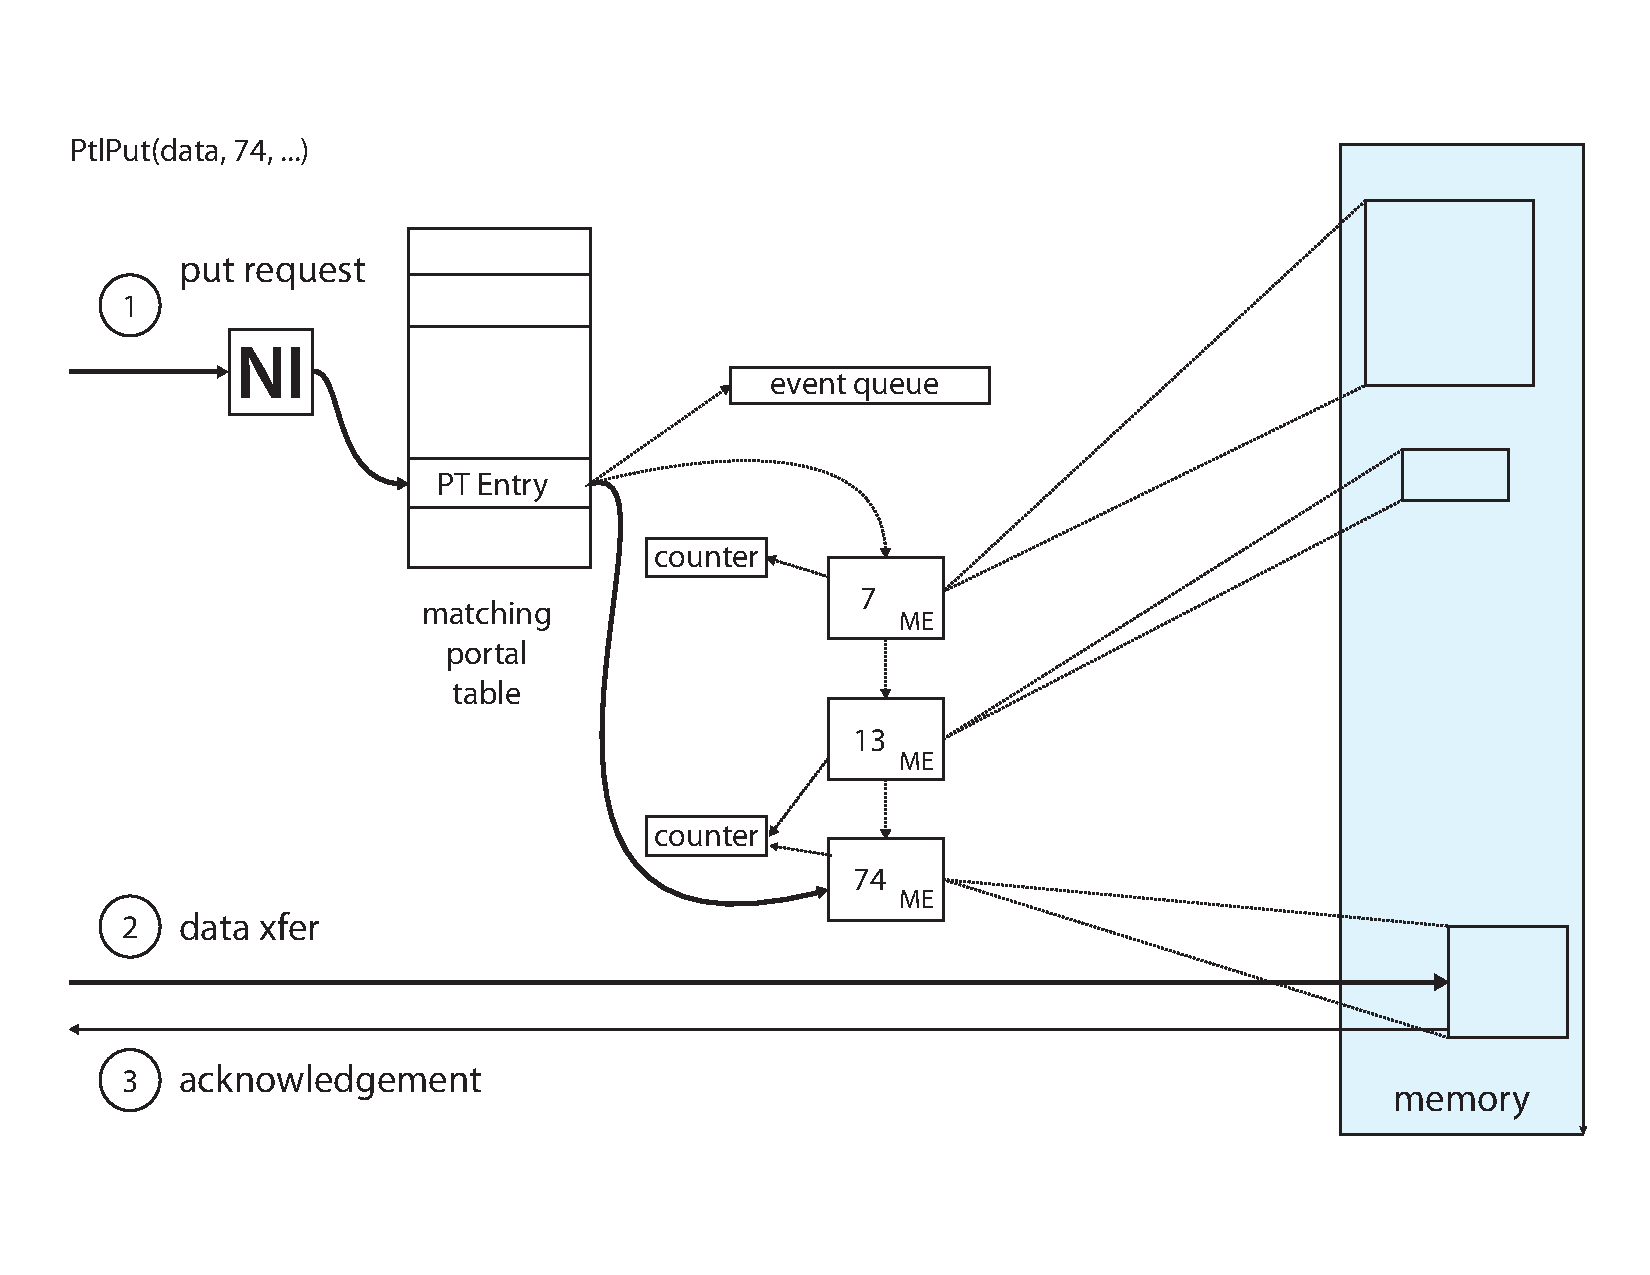
\includegraphics[width=\linewidth]{figs/portals_put}
  \caption{Portals data structures and example put operation.}
  \label{fig:portals_put}
\end{figure}

Portals defines two primary roles for communication operations. The
{\em initiator} is the process that is issuing the communication
request and the {\em target} is the process receiving the
requests. The initiator defines a {\em memory descriptor}, a
region to be used for Portals operations and is able to check the
success or failure of various events. Specific completion information
and notifications may be only visible to the initiator and not the
target, or vice versa.

Portals specifies a {\em network interface} (NI) as a per-process
abstraction of a physical network interface on the target process.The
interface is defined at creation to be either a {\em matching}
or a {\em non-matching} interface, depending on the intended use for
the interface (message-passing or one-sided). \pdht relies on the
Portals matching interface.

Each interface is associated with a portal table. An index into the
portal table is specified on every Portals communication operation and
is used to separate and classify different channels between endpoints.
Every portal table entry (PTE) maintains a list of memory regions that
are available for communication operations as well as an event queue
to track asynchronous notifications for ongoing communication.

A PTE using the matching interface maintains a list of match-list
entries (ME). Each ME specifies a set of matching criteria and a
memory region associated with the entry. If all of the match criteria
are satisfied, the communication operation commences working on
corresponding memory region. In particular, each ME contains a 64-bit
{\em match bits} field that must correspond to the match bits
specified on an incoming communication request. For example, a process
would post an {\tt MPI\_Recv()} with a specific match bits
field. Later, Portals would receive a communication request for an
{\tt MPI\_Send()} with the same match bits, which would be correspond
to the posted receive.

Additionally, Portals provides both {\em event queues} and {\em event
  counters} to track the data movement in and out of memory regions
used by Portals operations. Both events and counters are also used to
log failure events and other information. 

Events are detailed descriptions of communcation activities. They may
contain pointers to the transmitted data, send/receive parameters,
etc. An event queue may be associated with either the initiator
process or the target process.  On the initiator, an event queue may
be associated with the memory descriptor, whereas on the target,
an event queue may be associated with each PTE. 

Counters are useful for lightweight event counting, where copying a
large amount of data from the Portals implementation to the
application is unneccessary. Counters track the count of both
successful and failed communicadtion operations and are designed to
support efficient one-sided communication models. Like event queues, a
counter may be associated with either initiator or target
processes. Unlike target-side event queues, a counter may be
associated with each ME in the match-list. Multiple MEs may share a
single counter, if desired. \pdht typically uses counters to watch for
successful completion, and events to track specific failures. More
detailed descriptions of event and counter use within \pdht is
discussed below.

To put everything together, Figure \ref{fig:portals_put} shows the
relationships between the target-side data structures and a sample
{\tt PtlPut()} operation. In this example, we assume that the
initiator process has called {\tt PtlPut} with some data on a matching
interface, with the expected match bits set to 74. When the target
process receives the request, it is dispatched through the
initiator-specified PT index. Next, the match list is searched, until
a 74 is found, or the end of the list is reached. Once the ME has been
located, the PtlPut data is copied into the corresponding memory
region. The operation may cause a {\tt PUT} event to be appended to
the event queue or ME success counter to be incremented. An
acknowledgement is sent back to the initiator, possibly generating
another full event or counting event.



%reply: initiator: remote completion of a get: success = got it, failure = not
%found
%ack: initiator:  put completed
%put: target -> event with put data / ME
%flow control: initiator: disabled NI 

%%% Local Variables:
%%% mode: latex
%%% TeX-master: "paper"
%%% End:

\section{Implementation}

% serial vs. parallel approaches
Hash tables can be implemented with a myriad of different techniques,
but are traditionally implemented sequentially as an array of pointers to
objects. Parallel implementations typically distribute table data
across nodes, requiring that the hash table stores the entire object
and not simply a reference. 

\subsection{PDHT Programming Model}


% parallel programming model
%  - key/value pairs
%  - object can be located anywhere distributed memory, governed
%     solely by hash function
%  - hash function maps key -> rank/offset tuple
%  - two primary operations put/get
%     - if put yields a collision, then object is placed in next
%        available bucket
%     - get returns object, probing as necessary
 
The PDHT system provides a distributed key/value store within a
high-performance computing cluster. A hash function maps the object
key to a rank and offset tuple, identifying each distinct location
within the hash table. PDHT provides the two primary {\em put} and
{\em get} operations to store and fetch items from the table. Since
multiple keys may hash to the same table location (a collision), PDHT
implements a linear probing behavior. If a {\em put} yields a
collision, the object is then placed in the next available bucket on
the same processor rank. The {\em get} operation also checks for
collisions and searches accordingly. 

% considerations:
%  - two-sided communication not amenable to hash table implementation
%  - one-sided will rely on MPI-2+, UPC, or some other PGAS-ish
%     approach
Two-sided communication is not inherently amenable to implementing a
high-performance hash table. Hash tables rely on fine-grained, random
data access which makes a message-passing based implementation
challenging. Several existing approaches have been built upon
one-sided models using MPI-2, UPC, and other PGAS approaches.

\subsection{Portals 4}
% portals background
%  define NI, PTE
%  define matching, ME, matching lookup process
%  define counters and events

A primary motivation for using a one-sided approach is to allow
RDMA-based memory accesses to fetch remote data without interupting
the processor core on the far end. We can take advantage of NIC
hardware offload to a greater extent than conventional PGAS approaches
by using low-level communication primitives provided by the Portals 4
network interface specification. Portals defines a number of
abstractions and concepts that are necessary to understanding the PDHT
implementation.

Portals specifies a {\em network interface} (NI) as a per-process
abstraction of a physical network interface. Each NI is associated
with a portal table. The index into the portal table is specified on
every Portals communication operation and is used to separate and
classify different channels between endpoints.

Each portal table entry (PTE) maintains a list of memory regions that are
available for communication operations as well as an event queue to
track asynchronous notifications for ongoing communication. Portals
provides two distinct lists: {\em matching lists} that support
two-sided message passing systems and {\em non-matching lists} that
support one-sided communication models. PDHT relies on the matching
features of Portals and will be the focus of the remainder of the
implementation discussion.

A PTE using the matching interface maintains a list of match-list
entries (ME). Each ME specifies a set of matching criteria and a
memory region associated with the entry. If all of the match criteria
are satisfied, the communication operation commences working on
corresponding memory region. In particular, each ME contains a 64-bit
{\em match bits} field that must match exactly for an incoming
communication to proceed with the given ME. For example, a process
would post an {\tt MPI\_Recv()} with a specific match bits
field. Later, Portals would receive a communication request for an
{\tt MPI\_Send()} with the same match bits, which would be correspond
to the posted receive.

Additionally, Portals provides both {\em event queues} and {\em event
  counters} to track the data movement in and out of memory regions
used by Portals operations. Both events and counters are also used to
log failure events and other information.


\subsection{PDHT Implementation}

% use figure* to span both cols
\begin{figure}[ht]
  \centering
  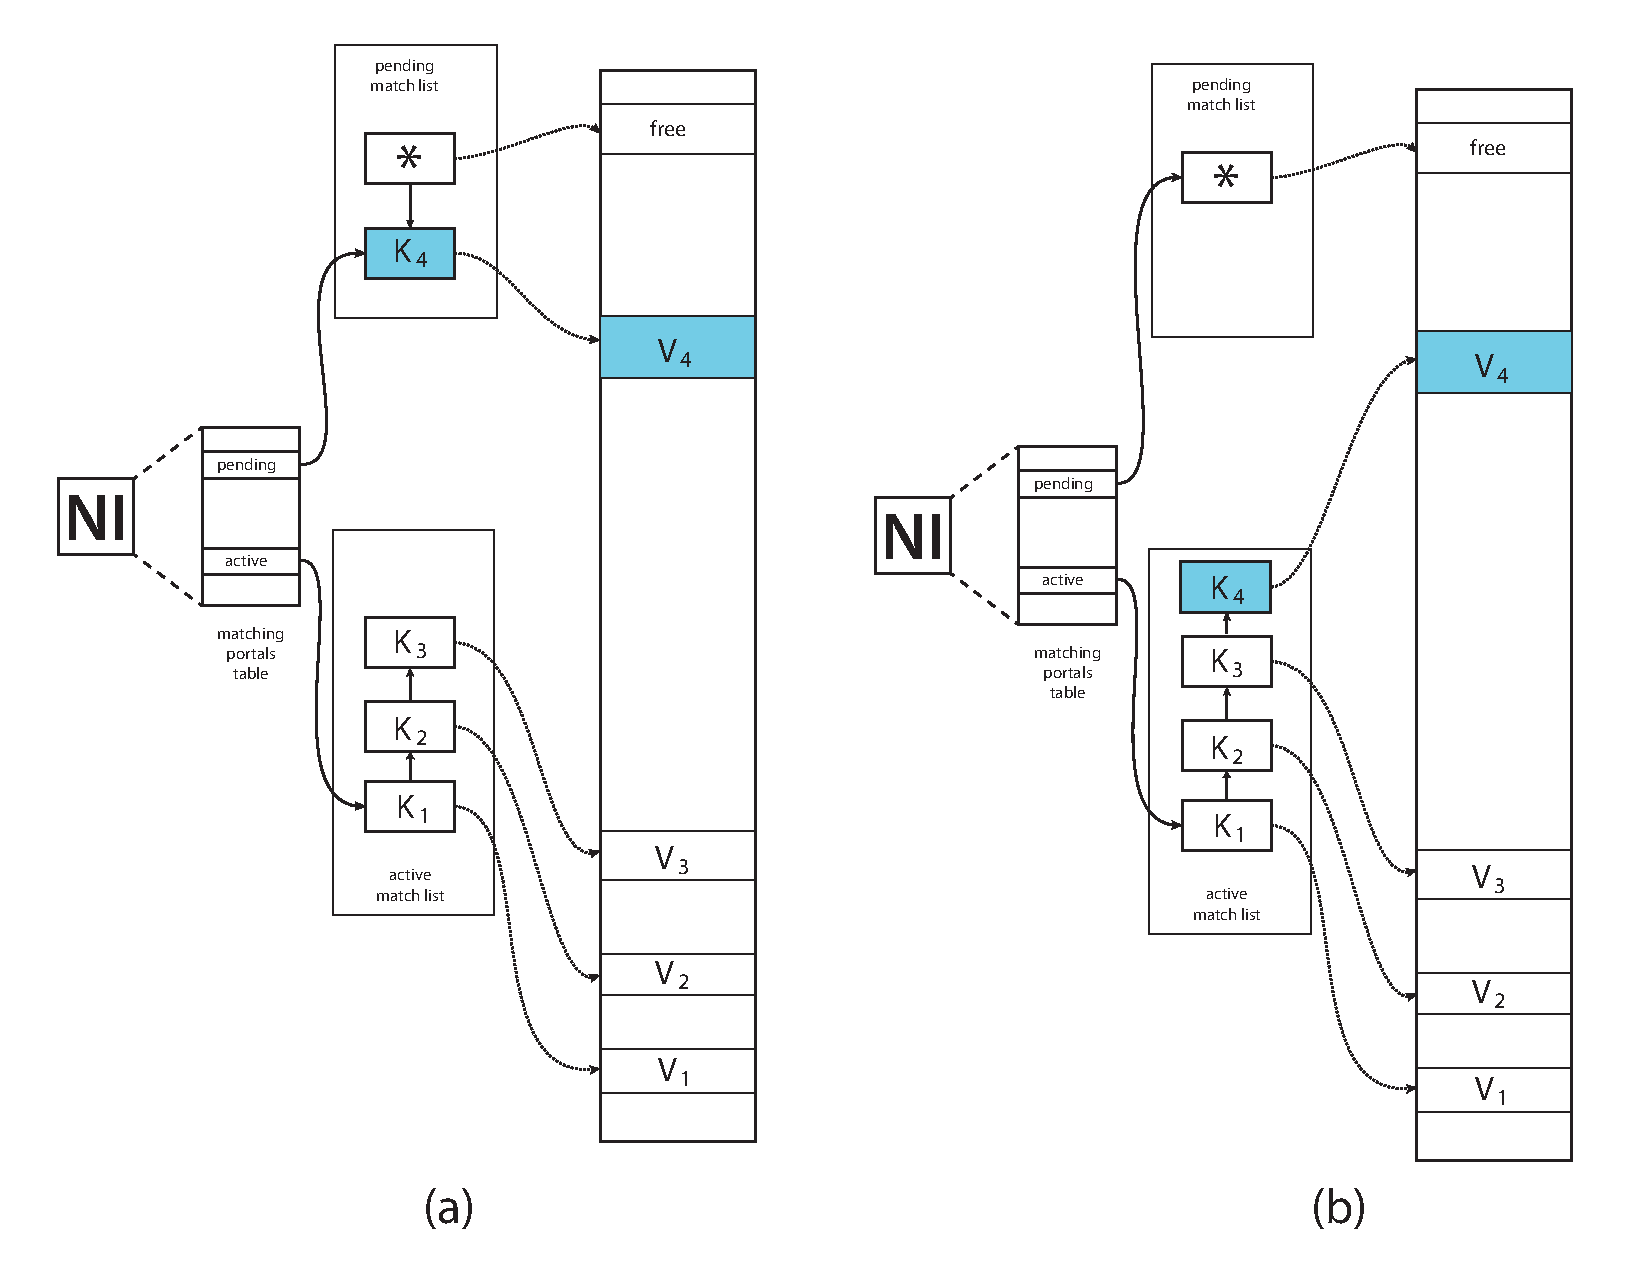
\includegraphics[width=3in]{figs/put_smaller}
  \caption{Slow motion {\tt put()} operation}
  \label{fig:put}
\end{figure}

\begin{figure}[ht]
  \centering
  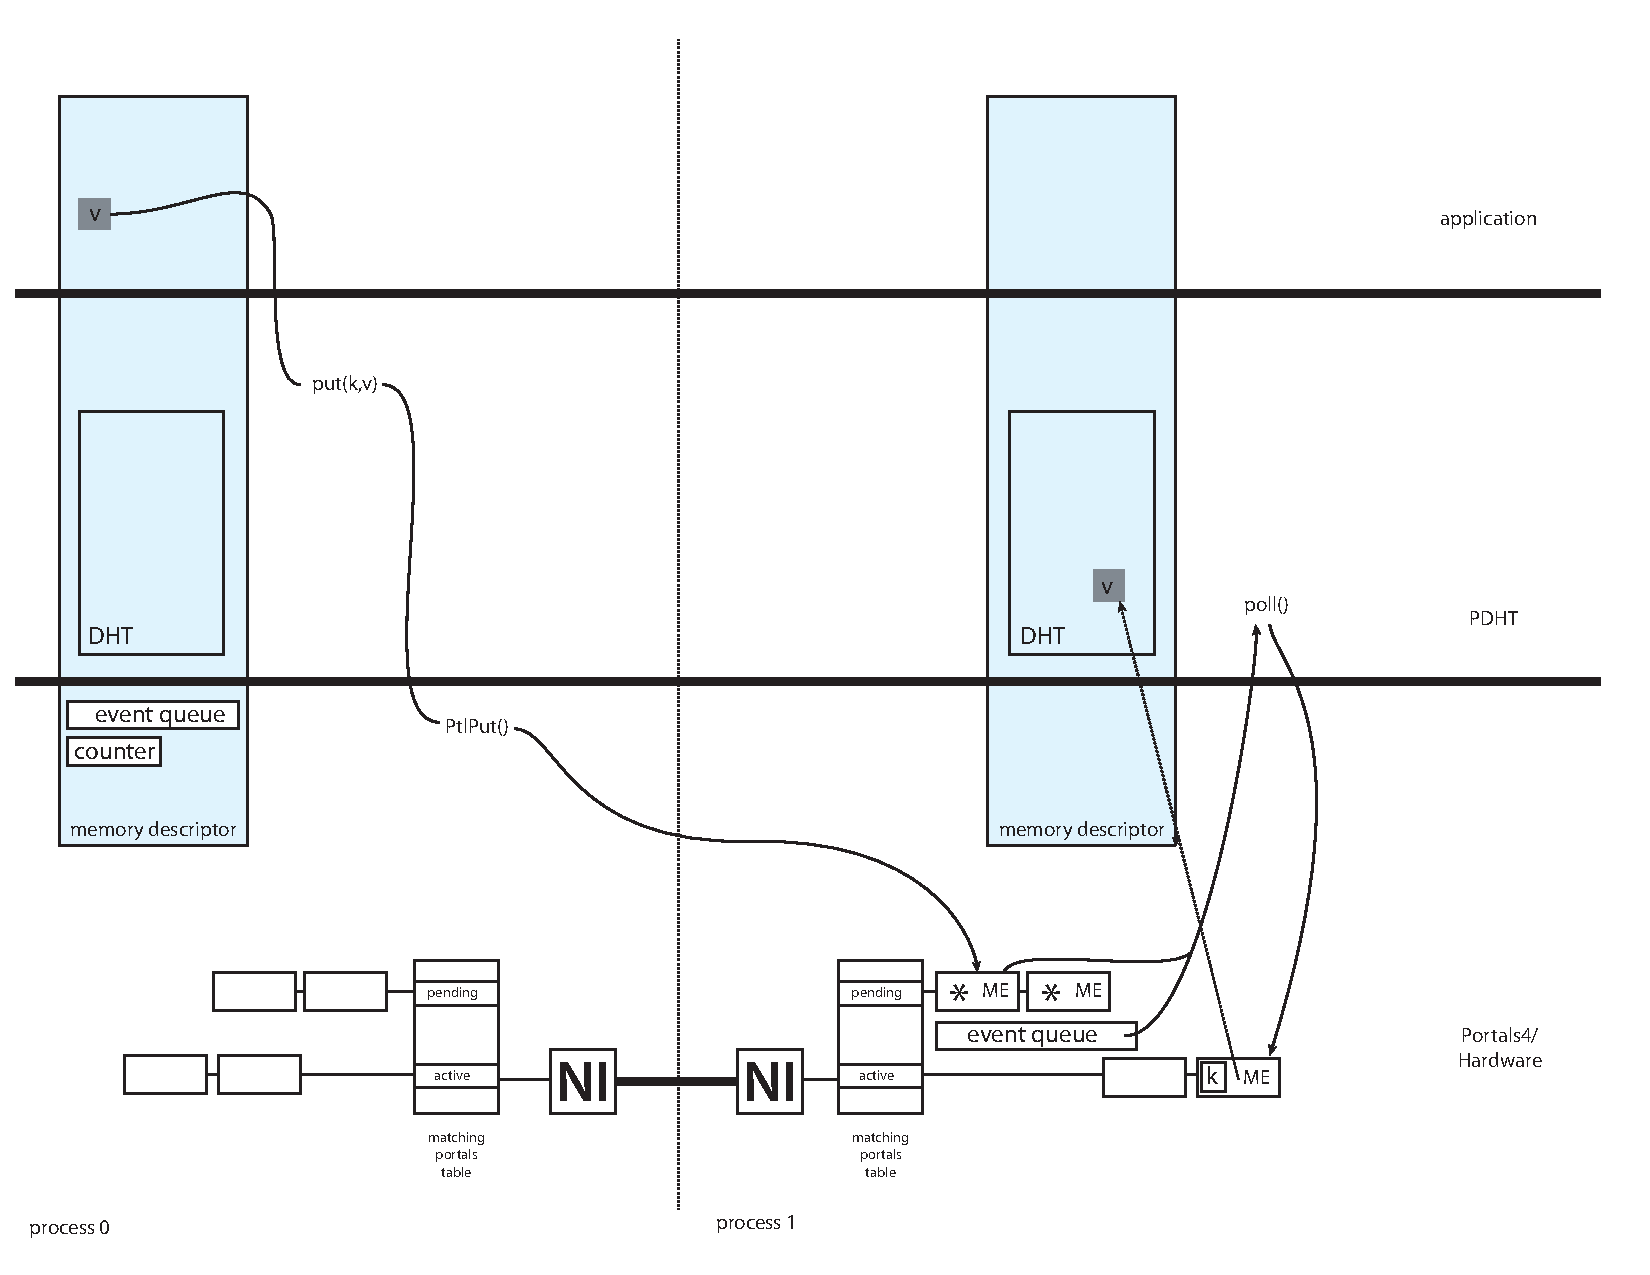
\includegraphics[width=3in]{figs/hwsw}
  \caption{Hardware/Software Abstractions}
  \label{fig:hwsw}
\end{figure}

% implementation
%  - array of objects + metadata
%  - pending ME list 
PDHT supports multiple hash tables per-process. Each hash table is
treated as a distributed array of value objects and a small amount of
metadata per entry. Upon initialization, PDHT opens a Portals NI with
two distinct portal table entries, one for {\em pending} match list
entries and another for {\em active} match list entries. The pending
match list is filled with a number of entries that will match any
incoming communication request. Each match list entry corresponds to a
local memory region that can contain a single entry in the hash table
array structure.

The key idea within PDHT is to create a match list entry (ME) for each
active element in the hash table. The hash function maps the key to a
64-bit value used as the match bits field for the Portals
communication request. By relying on the matching interface to handle
hash entries, much of the servicing of a get request can be relegated
to Portals, which in turn rely on hardware acceleration.

% put operation
%  - run hash to determine rank/offset
%  - figure 1
%  - active ME list
%  - migration from pending to active

To insert a new element into the hash table, the process first hashes
the key, giving both the target processor rank and the 64-bit match
bits field used for the value. Next, the process performs a one-sided
put operation on the pending PTE, using one of the wildcard entries on
the match list. The hash table value data is communicated and stored
into the memory region defined by the match list entry. As can be seen
in Figure \ref{fig:put}a, the table entry data resides on the owner
process, but the match-list entry is still resident on the pending
PTE, rather than the active one. To complete the put operation, the
used up entry on the pending PTE needs to be replaced with a new empty,
wildcard ME and the new hash table object needs to have an entry on
the active PTE, with the match bits set to correspond to the hashed
key. This state can be seen in Figure \ref{fig:put}b. 

% - polling approach
The most straightforward approach to moving the ME from the pending 
match list to the active list is by relying on a progress
thread. Portals provides blocking wait and polling routines to check
for new event notifications or counter changes. When a process
receives a put operation and updates the pending match list, a Portals
event is generated and appended to the event queue. When the progress
thread sees this event, it creates a replacement wildcard entry for
the pending queue that references an empty element in the hash table
array. It also creates a new ME with the appropriate match bits and
appends it to the active list. Any subsequent get requests will be
able to find a match in the active PTE.


% - triggered append approach


% get operation
%  - run hash
%  - issue PtlGet from active list
%  - check for collision


%  - custom hash functions 
%  - 64-bit hash space, rather than array bucket
%      - detach key -> array size dependency
%      - lower collision rates

% other operations
%  - iteration
%  - non-blocking / bundled puts/gets
%  - interoperability


%%% Local Variables: 
%%% mode: latex
%%% TeX-master: "paper"
%%% End: 

\section{Experimental Evaluation}
\label{sec:results}

We have gathered preliminary performance results using a prototype
implementation of \pdht running on the Portals reference
implementation~\cite{portals-code}.  Results were gathered on the Comet
system at the San Diego Supercomputer Center with access provided
through the Extreme Science and Engineering Discovery Environment (XSEDE)
program.  Comet contains nodes with several configurations; for our
experiments, we used the Intel\regtm Xeon\regtm E5 nodes.  There are 1944 such
nodes, which are constructed from Dell\othertm PowerEdge\othertm C6320 servers
containing dual 12-core Intel\regtm Xeon\regtm E5-2680 processors and 128
gigabytes of memory.  Nodes are connected using a Mellanox\othertm FDR 56 Gb/s
InfiniBand\othertm fabric.

As an initial proof point, we measure the performance of retrieving elements
from the \pdht in different scenarios.  These results are shown in
Figure~\ref{fig:mlen} and provide an initial characterization of the lookup
cost associated with our \pdht implementation.  In contrast with traditional
PGAS approaches, building a remotely accessible key/value store on top of a
mechanism intended to support MPI message matching can add new overheads.  In
particular, the Portals message processing engine must traverse the active
match list until an ME that matches the given query is located.  In cases where
the element does not exist, the Portals layer must reach the end of the list to
make this conclusion.  Thus, there is a list traversal overhead that is
proportional to the number of elements visited before finding a match.

\begin{figure}
    \centering
    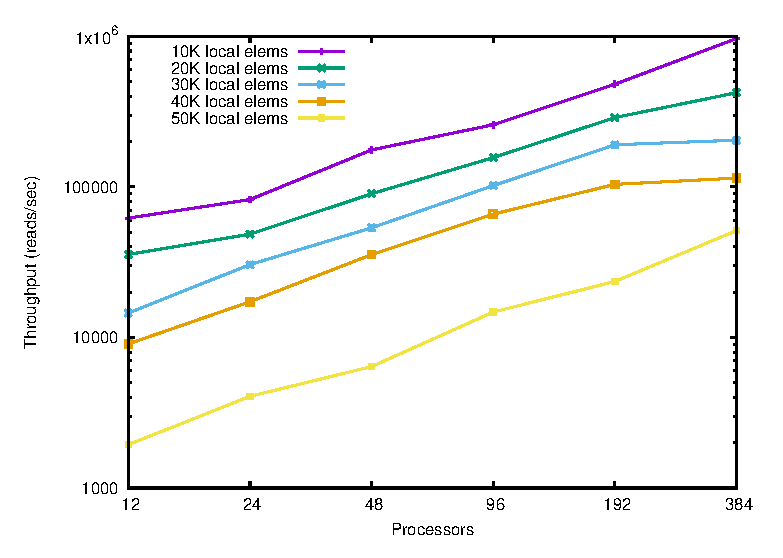
\includegraphics[width=\linewidth]{plots/throughput}
    \caption{System throughput for a range of local volume (entries per node).}
    \label{fig:throughput}
\end{figure}

\begin{figure}
    \centering
    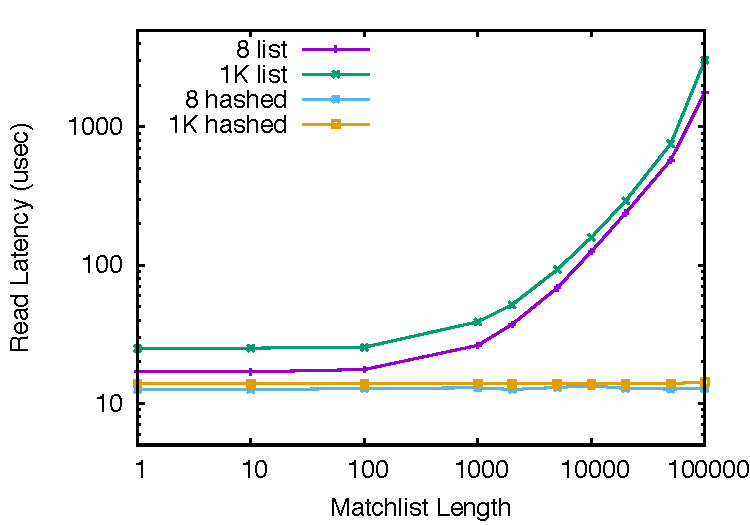
\includegraphics[width=\linewidth]{plots/mlen}
    \caption{Read operation latency versus list depth for various size entries.}
    \label{fig:mlen}
\end{figure}

The Portals layer must maintain each matching list as an ordered list in order
to preserve MPI message ordering semantics.  However, we observe that this
ordering is not required by \pdht.  Also, in contrast to MPI applications,
where typical communication patterns result in short matching lists or in
matching occurring near the head of the list, \pdht necessarily generates long
matching lists with an expected matching depth of the midpoint in the list.
Thus, we identify this overhead as a key challenge to supporting such models
and plan to investigate solutions in our future work.

%%% Local Variables:
%%% mode: latex
%%% TeX-master: "paper"
%%% End:

\section{Conclusion}

This paper has presented the partitioned global address space (PGLAS)
programming model and a functioning implementation of the model in
PDHT. The PDHT system makes novel use of the Portals networking interface
by re-purposing the message-matching system to operate as a key mechanism
for a global, distributed key/value store. We envision that a number of
applications that rely on sparse methods can be readily adapted to the PGLAS
parallel programming model and have demonstrated that such systems can 
result in good performance.

This work has led to several insights into adapting Portals data abstractions
onto higher-level programming models. In particular, the separation of the
message matching mechanics from the requirement for ordered delivery is
critical to good performance with PDHT. We see future opportunities for
adapting the Portals triggered operations with separate semantics for capturing
the trigger parameters at setup time versus invocation time evaluation. Lastly, 
this work has motivated the need for permitting applications to search
the priority list for matching.

\section*{Acknowledgement}

This work used the Extreme Science and Engineering Discovery Environment
(XSEDE), which is supported by National Science Foundation grant number
ACI-1053575.

We would also like to acknowledge Ryan Grant and Todd Kordenbrock at Sandia
National Laboratories for their help with Portals-related issues and the
generous use of Sandia test bed facilities as well as Evangelos Georganas at
Intel for his assistance with the Meraculous benchmark.


%\pagebreak

%\singlespacing
\bibliographystyle{ACM-Reference-Format}
%\bibliographystyle{IEEEtran}
\bibliography{bibdb}
%\input{appendix}
%\pagebreak
%\vfill
\begin{flushright}
%\scriptsize
\footnotesize
\framebox{
  \parbox{\columnwidth}
  {
  Intel and Xeon are trademarks of Intel Corporation in the U.S. and/or other countries.
  Software and workloads used in performance tests may have been optimized
  for performance only on Intel microprocessors.  Performance tests, such as
  SYSmark and MobileMark, are measured using specific computer systems,
  components, software, operations and functions.  Any change to any of those
  factors may cause the results to vary.  You should consult other information
  and performance tests to assist you in fully evaluating your contemplated
  purchases, including the performance of that product when combined with
  other products.  For more information go to \url{http://www.intel.com/performance}.
  }
}
%\normalsize
\end{flushright}
%~\\

\noindent\othertm{}{\footnotesize Other names and brands may be claimed as the
property of others.}

\end{document}
